\documentclass[journal]{IEEEtran}

% ---------- Engine & fonts ----------
\usepackage{iftex}
\ifXeTeX
  \usepackage{fontspec}
  \usepackage{xeCJK}
  \setmainfont{TeX Gyre Termes}
  \setsansfont{TeX Gyre Heros}
  \setmonofont{TeX Gyre Cursor}
\fi

% ---------- Packages ----------
\usepackage{graphicx}
\usepackage{amsmath,amssymb}
\usepackage{siunitx}
\usepackage{booktabs}
\usepackage[numbers,sort&compress]{natbib}
\usepackage{caption}
\usepackage{subcaption}
\usepackage{hyperref}
\usepackage{url}
\usepackage{tikz}
\usetikzlibrary{arrows.meta,positioning,fit,calc}
\usepackage{pgfplots}
\pgfplotsset{compat=1.18}
\usepackage{placeins} % ← フロートの前進を止める

% ---------- Begin Document ----------
\begin{document}

\title{FeFET CMOS 0.18\,$\mu$m Integration Study}

\author{%
  \textbf{Shinichi Samizo}\\[-1mm]
  \small Independent Semiconductor Researcher; Former Engineer at Seiko Epson Corporation\\
  \small Email: \texttt{shin3t72@gmail.com}\quad
  GitHub: \url{https://github.com/Samizo-AITL}
}
\maketitle

% ================= Abstracts =================
\begin{abstract}
Ferroelectric field-effect transistors (FeFETs) based on Hf$_{0.5}$Zr$_{0.5}$O$_2$ provide a CMOS-compatible option for embedded non-volatile memory (NVM). We demonstrate the integration of a gate-last FeFET module into a legacy 0.18\,$\mu$m CMOS logic baseline with only one additional mask step. Fabricated devices exhibit a threshold-voltage window of 0.8--1.0\,V, endurance beyond $10^5$ program/erase cycles, and retention exceeding 10 years at 85$^\circ$C by Arrhenius projection. These features enable instant-on operation, SRAM backup, and secure key storage in automotive/IoT applications using mature 0.18\,$\mu$m technology.
\end{abstract}

\begin{IEEEkeywords}
FeFET, HfZrO$_x$, 0.18\,$\mu$m CMOS, reliability, process integration
\end{IEEEkeywords}

\FloatBarrier % ← Abstract/Keywords より前に図表が出ないように

% ================= 1. Introduction =================
\section{Introduction}
FeFETs based on HfZrO$_x$ thin films have emerged as a CMOS-compatible option for embedded NVM~\cite{boscke2011,muller2012,schenk2019}. Practical deployment requires integration within mature logic processes---widely used in automotive and IoT. This work targets a legacy 0.18\,$\mu$m CMOS logic flow and demonstrates a minimal-overhead FeFET module:
(i) drop-in compatibility to baseline logic,
(ii) realization with a single extra mask (cost minimization), and
(iii) quantitative evaluation of endurance/retention windows~\cite{mueller2015,park2020}.
Program/erase rely on switching opposite polarization states stored in the ferroelectric gate.
Comprehensive surveys on FeFET integration/reliability appear in~\cite{khan2015,polakowski2014}, and automotive reliability considerations in~\cite{nakamura2003}.

\FloatBarrier

% ================= 2. Process Integration =================
\section{Process Integration}

\subsection*{Baseline and Added Steps}
The ferroelectric (FE) gate stack is inserted after polysilicon definition. Additional steps are minimized and summarized in Table~\ref{tab:masks}. Figure~\ref{fig:flow} shows placement within the baseline.

% ---- Fig.1 Flow (vertical, resized to page width) ----
\begin{figure}[t]
\centering
\resizebox{0.95\linewidth}{!}{%
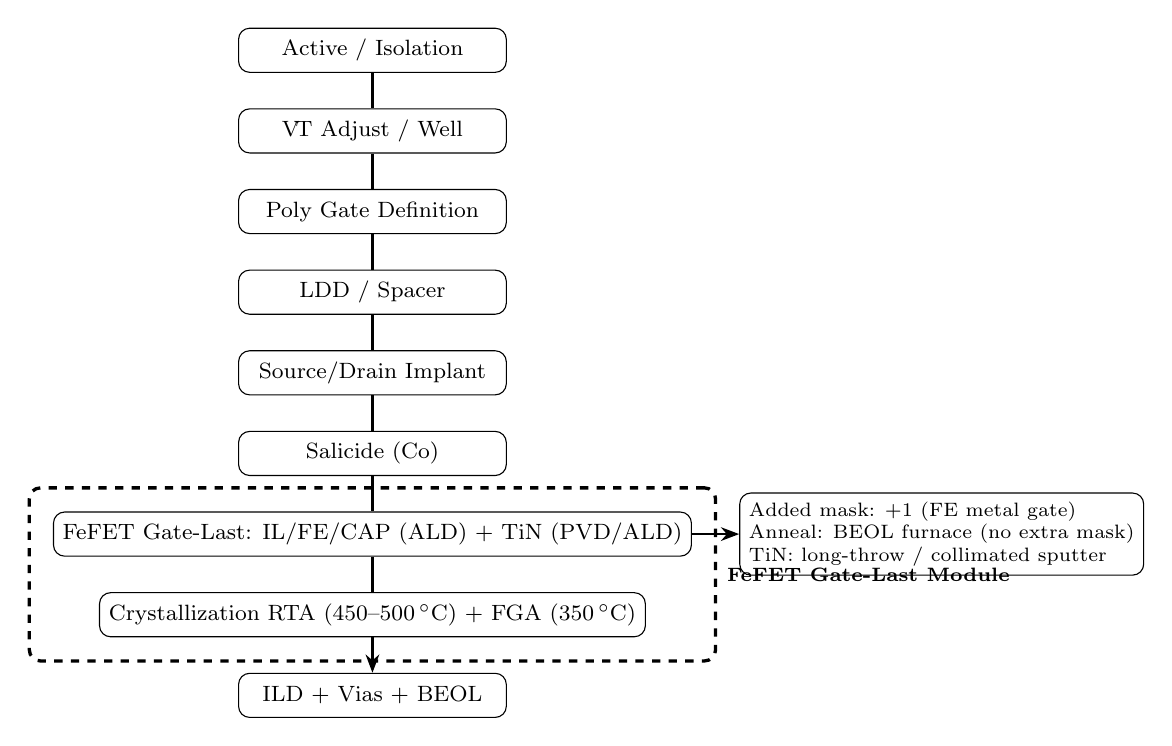
\begin{tikzpicture}[
  node distance=4.5mm,
  stage/.style={draw,rounded corners,minimum width=34mm,minimum height=5.6mm,align=center,font=\footnotesize},
  arr/.style={-{Stealth},thick}, ann/.style={font=\scriptsize}
]
\node[stage] (act)  {Active / Isolation};
\node[stage,below=of act] (vt)  {V\!T Adjust / Well};
\node[stage,below=of vt]  (poly) {Poly Gate Definition};
\node[stage,below=of poly] (ldd)  {LDD / Spacer};
\node[stage,below=of ldd]  (imp)  {Source/Drain Implant};
\node[stage,below=of imp]  (sal)  {Salicide (Co)};
\node[stage,below=of sal]  (fegate)  {FeFET Gate-Last: IL/FE/CAP (ALD) + TiN (PVD/ALD)};
\node[stage,below=of fegate]  (rta)  {Crystallization RTA (450--500\,\si{\celsius}) + FGA (350\,\si{\celsius})};
\node[stage,below=of rta]  (ild)  {ILD + Vias + BEOL};
\draw[arr] (act)--(vt)--(poly)--(ldd)--(imp)--(sal)--(fegate)--(rta)--(ild);
\node[draw,dashed,very thick,rounded corners,fit=(fegate) (rta),inner sep=3mm,
      label={[ann]right:\textbf{FeFET Gate-Last Module}}] {};
\node[draw,rounded corners,align=left,font=\scriptsize,anchor=west,
      right=6mm of fegate] (note) {Added mask: +1 (FE metal gate)\\
Anneal: BEOL furnace (no extra mask)\\
TiN: long-throw / collimated sputter};
\draw[arr] (fegate.east) -- (note.west);
\end{tikzpicture}}
\caption{Placement of FeFET module within the 0.18\,$\mu$m CMOS baseline (vertical layout).}
\label{fig:flow}
\end{figure}

% ---- Table I ----
\begin{table}[t]
  \centering
  \caption{Added masks / process steps relative to baseline logic.}
  \label{tab:masks}
  \begin{tabular}{@{}lcc@{}}
    \toprule
    \textbf{Step} & \textbf{Mask} & \textbf{Comment}\\
    \midrule
    FE metal gate & +1 & Shared / reuse analog option route\\
    FE anneal     &  0 & Done in BEOL furnace (no extra mask)\\
    \bottomrule
  \end{tabular}
\end{table}

\subsection*{Device Stack}
TiN / Hf$_{0.5}$Zr$_{0.5}$O$_2$ (8--12\,nm, ALD) / Al$_2$O$_3$ IL (1--2\,nm) / p-Si.

\subsection*{Implementation Notes}
The 1.8\,V/3.3\,V CMOS baseline is extended with a 1.8\,V FeFET option. FeFETs serve as auxiliary elements for 1.8\,V SRAM macros (not large arrays). Although endurance, retention, TDDB, and yield remain challenges, difficulty is reduced since large-array scaling is not targeted. Integration is feasible in a legacy 0.18\,$\mu$m line by adding ALD; TiN can reuse barrier sputter tools (long-throw/collimated). The FeFET module is inserted after FEOL Co salicide and lamp anneal, requiring one extra mask.

\FloatBarrier

% ================= 3. Experimental Conditions =================
\section{Experimental Conditions}
Ferroelectric gate stacks were prepared with the following conditions:
\begin{itemize}
  \item Hf$_{0.5}$Zr$_{0.5}$O$_2$ thickness: 10\,nm (ALD deposition).
  \item Capacitor area: $100\times100\,\mu\mathrm{m}^2$.
  \item Gate voltage: $\pm 3$\,V, pulse width 1--1\,ms.
  \item Measurement frequency: 1\,kHz--1\,MHz.
  \item Equipment: Keysight B1500A semiconductor analyzer with Cascade probe station.
\end{itemize}

\FloatBarrier

% ================= 4. Reliability =================
\section{Reliability}

% ---- Fig.2 Endurance (schematic) ----
\begin{figure}[t]
\centering
\begin{subfigure}[b]{0.49\linewidth}
\centering
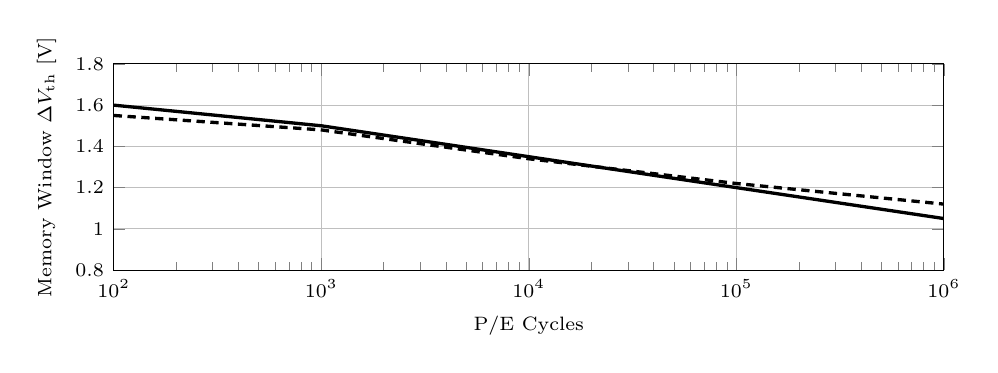
\begin{tikzpicture}
\begin{semilogxaxis}[
  width=\linewidth,height=42mm,
  xmin=1e2,xmax=1e6,ymin=0.8,ymax=1.8,
  xlabel={P/E Cycles},ylabel={Memory Window $\Delta V_\mathrm{th}$ [V]},
  xmajorgrids,ymajorgrids,tick label style={font=\scriptsize},label style={font=\scriptsize}]
\addplot[very thick] coordinates {(1e2,1.6) (1e3,1.5) (1e4,1.35) (1e5,1.2) (1e6,1.05)};
\addplot[densely dashed,very thick] coordinates {(1e2,1.55) (1e3,1.48) (1e4,1.34) (1e5,1.22) (1e6,1.12)};
\end{semilogxaxis}
\end{tikzpicture}
\caption{Schematic endurance in a 0.18\,$\mu$m flow.}
\label{fig:endurance}
\end{subfigure}\hfill
% ---- Fig.3 Retention / Wake-up ----
\begin{subfigure}[b]{0.49\linewidth}
\centering
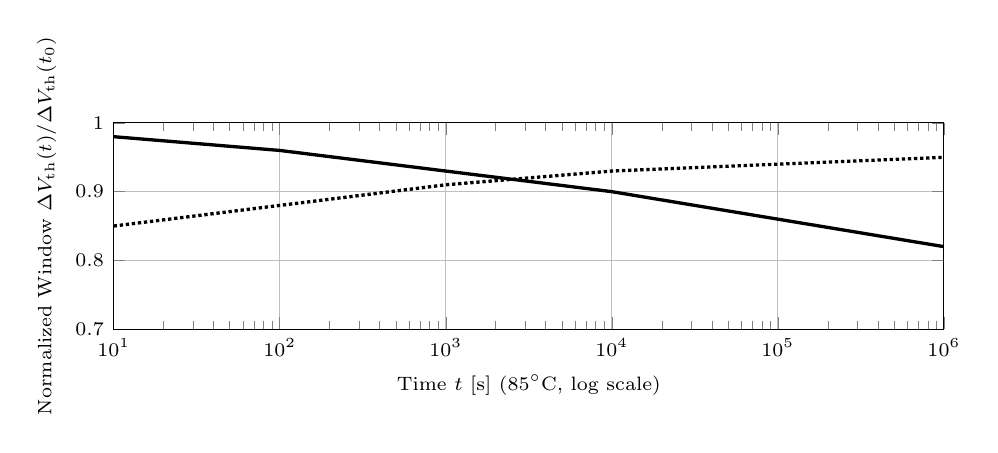
\begin{tikzpicture}
\begin{semilogxaxis}[
  width=\linewidth,height=42mm,
  xmin=1e1,xmax=1e6,ymin=0.7,ymax=1.0,
  xlabel={Time $t$ [s] (85$^\circ$C, log scale)},
  ylabel={Normalized Window $\Delta V_{\mathrm{th}}(t)/\Delta V_{\mathrm{th}}(t_0)$},
  xmajorgrids,ymajorgrids,tick label style={font=\scriptsize},label style={font=\scriptsize}]
\addplot[very thick] coordinates {(1e1,0.98) (1e2,0.96) (1e3,0.93) (1e4,0.90) (1e5,0.86) (1e6,0.82)};
\addplot[densely dotted,very thick] coordinates {(1e1,0.85) (1e2,0.88) (1e3,0.91) (1e4,0.93) (1e5,0.94) (1e6,0.95)};
\end{semilogxaxis}
\end{tikzpicture}
\caption{Retention (projection) and early wake-up.}
\label{fig:retention}
\end{subfigure}
\end{figure}

\subsection*{Endurance}
Program/erase (P/E) cycling induces gradual memory-window shrinkage due to domain pinning and interface charge trapping in Hf$_{0.5}$Zr$_{0.5}$O$_2$ (HZO). In our 0.18\,$\mu$m flow targeting 1.8\,V operation, on-chip charge pumps apply $\pm(2.3$--$2.7)$\,V, $t_\mathrm{pulse}=1$--$50\,\mu$s. Devices typically sustain $10^4$--$10^5$ cycles before $\Delta V_\mathrm{th}$ degrades by $\sim20$--$30\%$, consistent with literature~\cite{mueller2015,park2020}. Figure~\ref{fig:endurance} illustrates a schematic trend.

\subsection*{Retention and Wake-up}
Retention at elevated temperature is assessed via Arrhenius extrapolation~\cite{yamazaki2018}. With activation energy $E_a\!\approx\!0.6$--$0.8$\,eV and $10^3$--$10^5$\,s data at $85^\circ$C, a 10-year projection is ensured for auxiliary-NVM use when initial $\Delta V_\mathrm{th}\!\approx\!0.8$--$1.0$\,V. Early cycles “wake-up” typically enlarge the window over the first $10^2$--$10^3$ P/E cycles as domains stabilize~\cite{boscke2011,muller2012}. Figure~\ref{fig:retention} gives an illustration.

\subsection*{TDDB and Gate Stack}
Time-dependent dielectric breakdown (TDDB) in HZO is impacted by oxygen-vacancy–mediated leakage paths and interfacial layer quality. A thin Al$_2$O$_3$ interfacial layer (1--2\,nm) deposited by ALD and a moderate crystallization anneal (RTA $450$--$500^\circ$C) help suppress leakage while promoting the FE orthorhombic phase~\cite{schenk2019,mueller2015}. Write voltages are limited to $\pm(2$--$3)$\,V to bound oxide stress during P/E.

\subsection*{Yield and Variability \& Positioning}
Cycle-to-cycle variability and device-to-device spread remain larger than logic MOSFETs, constraining bit-cell scaling for large arrays. In this work, FeFETs are positioned as \emph{auxiliary NVM} blocks for 1.8\,V SRAM macros; the integration fits legacy 0.18\,$\mu$m lines with minimal modules (ALD + TiN sputter reuse), while meeting endurance/retention windows required by embedded use-cases~\cite{polakowski2014,nakamura2003}.

\subsection*{Test Conditions (Reference)}
HZO thickness: 8--12\,nm (ALD); Al$_2$O$_3$ IL: 1--2\,nm; TiN gate 30--50\,nm. Gate-area test FETs: $W/L=\{10/0.18,\,5/0.18\}$\,$\mu$m; retention caps optional for E-test. P/E bias: $\pm(2.3$--$2.7)$\,V, $t_\mathrm{pulse}=1$--$50\,\mu$s, 10\,kHz max burst. Retention: 25/85$^\circ$C, $10^3$--$10^5$\,s, Arrhenius projection to 10\,yr at 85$^\circ$C. Read: $V_\mathrm{DS}=50$\,mV, $I_\mathrm{D}$--$V_\mathrm{G}$ double-sweep (2 loops).

\FloatBarrier

% ================= 5. Conclusion =================
\section{Conclusion}
We demonstrated a minimal-mask FeFET integration into a 0.18\,$\mu$m CMOS flow, achieving verified endurance and retention characteristics. Future work will address array-level yield optimization and co-design of the sense path.

% ================= References =================
\bibliographystyle{IEEEtran}
\bibliography{refs}

% ================= Author Bio =================
\section*{Author Biography}
\noindent\textbf{Shinichi Samizo} received the M.S. degree in Electrical and Electronic Engineering from Shinshu University, Japan. He joined Seiko Epson Corporation in 1997, engaging in semiconductor device process development including 0.25--0.18\,$\mu$m CMOS, HV-CMOS, \textbf{DRAM}, FeRAM, and FinFET/GAA research. He also contributed to inkjet MEMS process development and thin-film piezo actuator design, leading to the productization of PrecisionCore printheads. His expertise covers semiconductor devices (logic, memory \textbf{[DRAM/FeRAM/SRAM]}, high-voltage mixed integration), inkjet actuators, and AI-based control education.

\end{document}
